\chapter{Perl概要}
\label{chap:chapterab}
\minitoc

本附录对Perl编程语言的相关内容进行了总结,这些知识对于你阅读本书大有裨益。它并不是对Perl语言进行的全面的总结。牢记一点,你不需要知道Perl的所有知识,就可以去使用它。本附录的原始材料是来源于\textit{Programming Perl, Third Edition} (O'Reilly \& Associates)的。

\section{命令解释}
本书中的Perl程序都起始于这样一行:

\begin{lstlisting}
#!/usr/bin/perl -w
\end{lstlisting}

在Unix(或Linux)系统中,文件的第一行可以包含程序的名称和一些可选的标志。该行必须以 \verb|#!|起始,后面紧跟程序(这我们的例子中,就是Perl解释器)的全路径\footnote{译者注:即绝对路径。}名,之后是可选的由一个或多个标志做成的标志组。

如果Perl程序文件名为\textit{myprogram},并且有可执行的权限,你直接键入 \verb|myprogram|(或者可能是 \verb|./myprogram|,或者是程序的绝对或相对路径名)就可以运行程序了。

Unix操作系统会启动由命令解释行指定的程序,并把文件中第一行之后的所有内容作为程序的输入。所以,在这个例子中,它会启动Perl解释器,并把文件中的程序交由Perl解释器来运行。

上述其实是在命令行中输入:

\begin{lstlisting}
/usr/bin/perl -w myprogram 
\end{lstlisting}

的一种简写。

\section{注释}
从\#起始,一直到该行的结尾都是注释的内容。注释会被Perl解释器忽略掉,它仅供程序员阅读。在注释中可以包含任何文本内容。

\section{标量值和标量变量}
一个标量值是数据的单一项目,比如一个字符串或者一个数字。

\subsection{字符串}
字符串是标量值,书写形式就是包裹在单引号内的文本,就像这样:

\begin{lstlisting}
'This is a string in single quotes.'
\end{lstlisting}

或者使用双引号,像这样:

\begin{lstlisting}
"This is a string in double quotes."
\end{lstlisting}

单引号包裹的字符串会被原样输出。使用双引号时,你可以在字符串中包含变量,在输出时变量的值会被插入或者“以内插值替换”。你还可以使用 \verb|\n|这样的命令来表示一个新行(参看\autoref{tab:tablea.b3}):

\begin{lstlisting}
$aside = '(or so they say)';
$declaration = "Misery\n $aside \nloves company.";
print $declaration;
\end{lstlisting}

这个代码片段会输出:

\begin{lstlisting}
Misery 
 (or so they say) 
loves company.
\end{lstlisting}

\subsection{数字}
数字可以是如下的标量值:

\begin{itemize}
  \item 整数:\\  \verb|3|\\  \verb|-4|\\  \verb|0|
  \item 浮点数(小数):\\  \verb|4.5326|
  \item 科学计数法(指数)($3.13 \times 10^{23}$或313000000000000000000000):\\  \verb|3.13E23|
  \item 十六进制(以16为基数):\\  \verb|Ox12bc3|
  \item 八进制(以8为基数):\\  \verb|O5777|
  \item 二进制(以2为基数):\\  \verb|0b10101011|
\end{itemize}

 \verb|3 + i|这样的复数(或虚数),以及 \verb|1/3|这样的分数(或比率,或有理数),使用起来会有点麻烦。Perl可以处理分数,但在内部会把它们转换成浮点数,这会使某些操作符出现错误(计算机语言中存在该问题的不仅仅是Perl):

\begin{lstlisting}
if ( 10/3  == ( (1/3) * 10  ) {
  print "Success!";
}else {
  print "Failure!";
}
\end{lstlisting}

这会输出:

\begin{lstlisting}
Failure!
\end{lstlisting}

要准确地处理分数、复数或其他许多数学结构的有理运算,可以使用相应的数学模块,此处不进行赘述。

\subsection{标量变量}
标量值可以存储在标量变量中。一个标量变量用变量名前面的 \verb|$|来进行表明。变量名以字母或下划线起始,可以包含任意数量的字母、下划线和数字。但是,数字不可以是变量名的第一个字符。下面是标量变量合法名称的一些例子:

\begin{lstlisting}
$Var
$var_1
\end{lstlisting}

下面是变量变量的一些不合法的名称:

\begin{lstlisting}
$1var
$var!iable
\end{lstlisting}

变量名是大小写敏感的: \verb|$dna|和 \verb|$DNA|是两个不同的变量。

这些用来生成合法标量变量名的规则(除以 \verb|$|起始外),同样适用于数组和散列的变量名,以及子程序的命名。

一个标量变量可能存储前面提到的任意一种变量值,比如字符串或者不同类型的数字。

\section{赋值}
使用赋值语句,把标量值赋值给标量变量。例如:

\begin{lstlisting}
$thousand = 1000;
\end{lstlisting}

把1,000这个标量值赋值给了标量变量 \verb|$thousand|。

赋值语句和初等数学里面的等号看起来非常相似,但意义完全不同。赋值语句是一个操作指令,而不是一个论断。它表示的不是“ \verb|$thousand|等于1,000”,而是“把标量值1,000存储到标量变量 \verb|$thousand|中去”。不管怎样,在这个语句执行后,标量变量 \verb|$thousand|的值确实等于1,000了。

你可以把多个值赋值给多个标量变量,方法就是把变量和值包裹在括号中并用逗号分隔开来,这实际上是构造了列表:

\begin{lstlisting}
($one, $two, $three) = ( 1, 2, 3 );
\end{lstlisting}

除了 \verb|=|以外,还有许多复制操作符,它们都是长表达式的简写。比如, \verb|$a += $b|等同于 \verb|$a = $a + $b|。\autoref{tab:tablea.b1}给出了完整的列表(它包含了本书中没有提到的一些操作符)。

\begin{table}[!htbp]
  \begin{center}
  \caption{复制操作符简写}
  \label{tab:tablea.b1}
  %\begin{tabu}{X[1,c]X[2,l]}
    \begin{tabu*} to 0.7\linewidth {X[1,c,m]X[3,l,m]}
    \toprule
    操作符实例 & 等同于\\
    \midrule
     \verb|$a += $b| &  \verb|$a = $a + $b| (加法)\\
     \verb|$a -= $b| &  \verb|$a = $a - $b| (减法)\\
     \verb|$a *= $b| &  \verb|$a = $a * $b| (乘法)\\
     \verb|$a /= $b| &  \verb|$a = $a / $b| (除法)\\
     \verb|$a **= $b| &  \verb|$a = $a ** $b| (求幂)\\
     \verb|$a |\% \verb|= $b| &  \verb|$a = $a |\% \verb| $b| (取模, \verb|$a/$b|的余数))\\
     \verb|$a x= $b| &  \verb|$a = $a x $b| (把字符串 \verb|$a|重复 \verb|$b|次)\\
     \verb|$a &= $b| &  \verb|$a = $a & $b| (位与)\\
     \verb+$a |= $b+ &  \verb+$a = $a | $b+ (位或)\\
     \verb|$a ^= $b| &  \verb|$a = $a ^ $b| (位异或)\\
     \verb|$a >>= $b| &  \verb|$a = $a >> $b| ( \verb|$a|右移 \verb|$b|位)\\
     \verb|$a <<= $b| &  \verb|$a = $a << $b| ( \verb|$a|左移 \verb|$b|位)\\
     \verb|$a &&= $b| &  \verb|$a = $a && $b| (逻辑与)\\
     \verb+$a ||= $b+ &  \verb+$a = $a || $b+ (逻辑或)\\
     \verb|$a .= $b| &  \verb|$a = $a . $b| (把字符串 \verb|$b|附加到 \verb|$a|后)\\
    \bottomrule
    \end{tabu*}
  \end{center}
\end{table}

\section{语句和块}
程序是由语句构成的,而语句通常组合成块。

语句以分号(;)结束,而对于块中的最后一个语句来说分号是可有可无的。

一个块通常就是用大括号包裹起来的一个或多个语句。下面是一个例子:

\begin{lstlisting}
{
  $thousand = 1000;
  print $thousand;
}
\end{lstlisting}

块可以独立存在,但通常都会与循环或 \verb|if|语句结构关联在一起。

\section{数组}
数组是有序的零个或多个标量值的集合,通过位置进行索引。一个数组变量起始于一个 \verb|@|符号,后面是一个合法的变量名。比如,下面是两个可能的数组变量名:

\begin{lstlisting}
@array1
@dna_fragments
\end{lstlisting}

你可以把标量值赋值给数组,方法就是把这些标量值放在列表中,用逗号分隔开、并用成对的括号包裹起来。比如,你可以把空列表赋值给数组:

\begin{lstlisting}
@array = ( );
\end{lstlisting}

或者,把一个或多个标量值赋值给数组:

\begin{lstlisting}
@dna_fragments = ('ACGT', $fragment2, 'GGCGGA');
\end{lstlisting}

注意,在一个列表中,完全可以指定像 \verb|$fragment2|这样的一个标量变量。存放到数组中的,是它现在的值,而非变量名。

数组中单个的标量值(元素)通过它们在数组中的位置进行索引。索引数组从0开始。在数组名前面使用 \verb|$|,在其后面紧跟用中括号 \verb|[ ]|包裹起来的元素索引数字,这样你就可以指定数组中特定的一个元素了,就想这样:

\begin{lstlisting}
$dna_fragments[2]
\end{lstlisting}

考虑到先前对数组进行的赋值,它现在的值就等于' \verb|GGCGGA|'。注意数组有三个标量值,分别用0、1和2进行索引。第三个、也就是最后一个元素的索引值是2,比总的元素数目3小1,这是因为第一个元素的索引值是0。

使用复制操作符 \verb|=|,你可以把数组复制一份,就像下面这个例子中一样,它为现有的数组 \verb|@input|复制了一份拷贝 \verb|@output|:

\begin{lstlisting}
@output = @input;
\end{lstlisting}

如果你在标量上下文中对数组进行求值,得到的值是数组中元素的数目。所以如果数组 \verb|@input|有五个元素,下面的这个例子就会把5这个值赋值给 \verb|$count|:

\begin{lstlisting}
$count = @input;
\end{lstlisting}

\autoref{fig:figurea.b1}展示了含有三个元素的数组 \verb|@myarray|,它演示了数组的有序属性。对于其中的每一个元素,都可以通过它在数组中的位置找到。

\begin{figure}
  \centering
  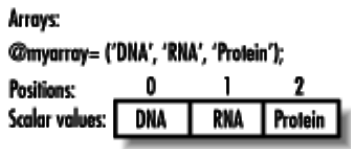
\includegraphics[width=0.5\textwidth]{figurea.b1.png}
  \caption{图解数组}
  \label{fig:figurea.b1}
 \end{figure}{}

\section{散列}
散列(也叫做关联数组)是零个或多个成对标量值的集合,这些成对的标量值叫做键和值。其中的值通过键进行索引。一个散列标量起始于一个 \verb|%|符号,后面是一个合法的变量名。比如,可能的散列变量名:

\begin{lstlisting}
%hash1
%genes_by_name
\end{lstlisting}

你可以使用一个简单的赋值语句把值赋值给键。比如,假设你有一个叫做 \verb|%baseball_stadiums|散列和一个叫做 \verb|Phillies|的键,你想把值 \verb|Veterans Stadium|赋值给这个键。下面的这个语句就可以完成赋值:

\begin{lstlisting}
$baseball_stadiums{'Phillies'} = 'Veterans Stadium';
\end{lstlisting}

注意,单独的一个散列值用散列名前面的 \verb|$|而非 \verb|%|进行指代;这和数组中使用的方法非常类似,当指代单独的一个数组值时使用 \verb|$|而非 \verb|@|。

你可以把多个键、值赋值给散列,方法就是把它们的标量值放在列表中,用逗号分隔开、并用成对的括号把它们包裹起来。每一个连续的标量对都会称为散列中的一个键和一个值。比如,你可以把空列表赋值给散列:

\begin{lstlisting}
%hash = ( );
\end{lstlisting}

你也可以把一个或多个标量键-值对赋值给散列:

\begin{lstlisting}
%genes_by_name = ('gene1', 'AACCCGGTTGGTT', 'gene2', 'CCTTTCGGAAGGTC');
\end{lstlisting}

还有另一种方法也可以完成同样的事情,但它使得键-值对的关系更加一目了然。下面做的事情和前面的例子完全一样:

\begin{lstlisting}
%genes_by_name = (
  'gene1' => 'AACCCGGTTGGTT',
  'gene2' => 'CCTTTCGGAAGGTC'
);
\end{lstlisting}

要提取和某个特定键相关联的值,只需要在散列名前使用 \verb|$|,并在其后紧跟包裹键的标量值的成对大括号 \verb|{ }|即可:

\begin{lstlisting}
$genes_by_name{'gene1'}
\end{lstlisting}

考虑到先前在散列 \verb|%genes_by_name|中对' \verb|gene1|'进行的赋值,它会返回' \verb|AACCCGGTTGGTT|'这个值。\autoref{fig:figurea.b2}展示了一个含有三个键的散列。

\begin{figure}
  \centering
  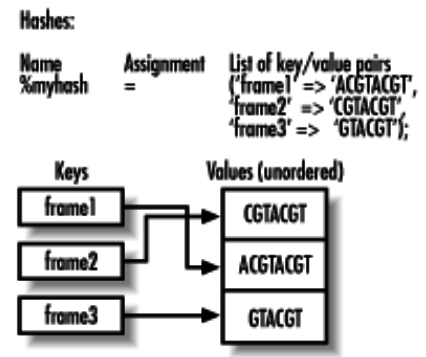
\includegraphics[width=0.7\textwidth]{figurea.b2.png}
  \caption{图解散列}
  \label{fig:figurea.b2}
 \end{figure}{}

\section{操作符}
操作符是代表对值进行加减等基本操作的函数。它们的使用非常频繁,是Perl编程语言的核心部分。它们其实就是需要参数的函数。举个例子, \verb|+|是把两个数进行相加的操作符,就像这样:

\begin{lstlisting}
3 + 4;
\end{lstlisting}

操作符通常有一个、两个或三个运算对象。在刚才的例子中,有 \verb|3|和 \verb|4|这么两个运算对象。

操作符可以出现在它们的运算对象的前面、中间或者后面。比如,加法运算符 \verb|+|就出现在它的运算对象的中间。

\section{操作符优先级}
操作符优先级决定了运算的顺序。比如,在Perl中,下面这个表达式:

\begin{lstlisting}
3 + 3 * 4
\end{lstlisting}

并不是从左到右进行求值的,也就是说,并不是先计算3加3等于6、然后把6乘以4得到24这个值的。优先级规则决定先乘法后加法,最终得到15这个结果。在\textit{perlop}手册页和大多数Perl书籍中都可以找到优先级规则。但是,我建议你使用括号来使你的代码更加易读,同时避免bugs。它们使得表达式清晰明确。第一个例子:

\begin{lstlisting}
(3 + 3) * 4
\end{lstlisting}

求值后得到24,而第二个例子:

\begin{lstlisting}
3 + (3 * 4)
\end{lstlisting}

求之后得到15。

\section{基本操作符}
关于操作符运算的更多信息,请查阅和Perl绑定在一起的 \verb|perlop|文档。

\subsection{算术操作符}
Perl有五个基本的算术操作符:

\noindent
\textcolor{red}{+}
\begin{adjustwidth}{4em}{}
加法
\end{adjustwidth}
\textcolor{red}{-}
\begin{adjustwidth}{4em}{}
减法
\end{adjustwidth}
\textcolor{red}{*}
\begin{adjustwidth}{4em}{}
乘法
\end{adjustwidth}
\textcolor{red}{/}
\begin{adjustwidth}{4em}{}
除法
\end{adjustwidth}
\textcolor{red}{**}
\begin{adjustwidth}{4em}{}
求幂
\end{adjustwidth}

这些操作符对整数和浮点数值都适用(如果你不小心地话,也可以对字符串使用)。

Perl还有一个 \verb|取模|操作符,它会计算两个整数的余数:

\begin{lstlisting}
% modulus
\end{lstlisting}

比如, \verb|17 % 3|的值为2,因为当你把17除以3后得到的余数是2。

Perl还有自增和自减操作符:

\begin{lstlisting}
++ 加一
-- 减一
\end{lstlisting}

和前面的六个操作符不同,它们会改变变量的值。 \verb|$x++|会给 \verb|$x|加一,把值从4变到5(或者从a变到b)。

\subsection{位操作符}
所有的标量,不管是数字还是字符串,“在底层”都是用一串单个的位(比特)来表示的。偶尔你需要操作这些位,而Perl提供了五个操作符可供使用:

\noindent
\textcolor{red}{\&}
\begin{adjustwidth}{4em}{}
位与
\end{adjustwidth}
\textcolor{red}{|}
\begin{adjustwidth}{4em}{}
位或
\end{adjustwidth}
\textcolor{red}{\^{}}
\begin{adjustwidth}{4em}{}
位异或
\end{adjustwidth}
\textcolor{red}{\textgreater\textgreater}
\begin{adjustwidth}{4em}{}
右移
\end{adjustwidth}
\textcolor{red}{\textless\textless}
\begin{adjustwidth}{4em}{}
左移
\end{adjustwidth}

\subsection{字符串操作符}
使用点操作符,可以把字符串连接起来——头尾相连:

\begin{lstlisting}
'This is a ' . 'joined string'
\end{lstlisting}

这会得到' \verb|This is a joined string|'这个值。

使用 \verb|x|操作符也可以把一个字符串进行重复:

\begin{lstlisting}
print "Hear ye! " x 3;
\end{lstlisting}

这会输出:

\begin{lstlisting}
Hear ye! Hear ye! Hear ye!
\end{lstlisting}

\subsection{文件测试操作符}
文件测试操作符是一元操作符,它会检测文件的特定属性,比如对于 \verb|-e $file|,当文件\textit{\$file}存在时它会返回 \verb|真|。\autoref{tab:tablea.b2}列出了一些可用的文件测试操作符。

\begin{table}[!htbp]
  \begin{center}
  \caption{文件测试操作符}
  \label{tab:tablea.b2}
    \begin{tabu*} to 0.8\linewidth {X[1,c,m]X[5,l,m]}
    \toprule
    操作符 & 含义\\
    \midrule
    -r & 文件是可读的\\
    -w & 文件是可写的\\
    -x & 文件是可执行的\\
    -o & 文件为“你”所有\\
    -e & 文件存在\\
    -z & 文件字节单位的大小为零\\
    -s & 文件的大小非零(返回以字节为单位的大小)\\
    -f & 文件是一个普通文件\\
    -d & 文件是一个目录(也就是文件夹)\\
    -l & 文件是一个符号链接\\
    -t & 文件句柄打开的是终端\\
    -T & 文件是一个文本文件\\
    -B & 文件是一个二进制文件\\
    -M & 文件最后一次被修改后至今(程序启动时)的天数\\
    -A & 文件最后一次被访问后至今(程序启动时)的天数\\
    -C & 文件最后一次节点编号被变更后至今(程序启动时)的天数\\
    \bottomrule
    \end{tabu*}
  \end{center}
\end{table}


\section{条件和逻辑操作符}
本节涵盖条件语句和逻辑操作符的相关内容。

\subsection{真和假}
在条件测试中,一个表达式求值的结果为 \verb|true|(真)或 \verb|false|(假)。基于求值结果的不同,一个语句或者代码块有可能执行,也有可能不执行。

在条件中,一个标量的值可能为 \verb|true|(真)或 \verb|false|(假)。如果一个字符串是空字符串(用""或''表示),那么它的值就为 \verb|false|;如果字符串不是空字符串,那么它的值就为 \verb|true|。

与之类似,如果一个数组或者散列为空,它的值就是 \verb|false|,不为空值就是 \verb|true|。

如果一个数字是0,它的值就为 \verb|false|;数字不是0,值就为 \verb|true|。

在Perl中,大多数东西在求值后都会返回一些值(比如:算数运算表达式返回的数字,或者子程序返回的数组),因此你可以在Perl的条件测试中使用它们。有时,你可能会得到一个未定义的值,例如当你把一个数字和一个还没有赋值的变量相加时,此时一切就会可能和预期相差甚远。举个例子:

\begin{lstlisting}
use strict;
use warnings;
my $a;
my $b;
$b = $a + 2;
\end{lstlisting}

会得到警告:

\begin{lstlisting}
Use of uninitialized value in addition (+) at - line 5.
\end{lstlisting}

使用Perl的函数 \verb|defined|来检测值是定义的还是未定义的。

\subsection{逻辑操作符}
一共有四种逻辑操作符:

\begin{lstlisting}
not
and
or
xor
\end{lstlisting}

 \verb|not|(非)会把 \verb|true|(真)值变 \verb|false|(假),把 \verb|false|(假)值变 \verb|true|(真)。用代码来更好的阐释以下:

\begin{lstlisting}
if(not $done) {...}
\end{lstlisting}

只有在 \verb|$done|的值为 \verb|false|(假)时,代码才会执行。

 \verb|and|(与)是一个二元操作符,只有当两边操作数的值都为 \verb|true|(真)时,它才会返回 \verb|true|(真)。如果有一个操作数为 \verb|false|(假),运算符都会返回 \verb|false|(假):

\begin{lstlisting}
1   and  1    returns true
'a' and  ''   returns false
''  and  0    returns false
\end{lstlisting}

 \verb|or|(或)也是一个二元操作符,只要两个操作数中至少有一个为 \verb|true|(真),它就会返回 \verb|true|(真)。如果两个操作数都为 \verb|false|(假),它会返回 \verb|false|(假):

\begin{lstlisting}
1   or  1    returns true
'a' or  ''   returns true
''  or  0    returns false
\end{lstlisting}

 \verb|xor|(异或)只有在两个操作数中一个为 \verb|true|(真)一个为 \verb|false|(假)的情况下才会返回 \verb|true|(真)。如果两个都为 \verb|true|(真)或者都为 \verb|false|, \verb|xor|会返回 \verb|false|(假):

\begin{lstlisting}
1 xor 0   returns true
0 xor 1   returns true
1 xor 1   returns false
0 xor 0   returns false
\end{lstlisting}

这几个操作符大多数都有变体:

\begin{lstlisting}
! for not
&& for and
|| for or
\end{lstlisting}

除了优先级不同以外,其他没有什么区别。一些老版本的Perl可能只有:

\begin{lstlisting}
!
||
&&
\end{lstlisting}

而没有 \verb|not|或者 \verb|and|。

\subsection{使用逻辑操作符控制流程}
要想依据上一个动作的结果来决定下一步的动作,最简便也是最流行的做法就是用逻辑操作符把语句链接组合在一起。比如,在Perl程序中,用来打开文件的下面这一个语句就非常常见:

\begin{lstlisting}
open(FH, $filename) or die "Cannot open file $filename: $!";
\end{lstlisting}

这个语句中 \verb|or|的使用展示了关于二元逻辑操作符的另一个重要的事情:它们是从左向右对参数进行求值的。在这个例子中,如果文件打开成功, \verb|or|操作符永远都不会去检查第二个操作数的值( \verb|die|会输出字符串中的信息并退出程序,如果使用了 \verb|$!|还会有一些额外的信息)。之所以会这样,是因为如果一个操作数为 \verb|true|(真), \verb|or|就为 \verb|true|,所以它根本不需要去检查第二个操作数的值。然而,如果文件打开失败, \verb|or|就需要去检查一下第二个操作数的值是 \verb|true|还是 \verb|false|,所以它就会继续执行 \verb|die|语句。

与之类似,你也可以使用 \verb|and|语句,在只有第一个操作成功的情况下才去测试第二个操作。

 \verb|xor|不会用于控制流程,因为每次都要对它的两个参数进行求值。

对于这种逻辑操作符控制的流程链我使用的并不多,我主要使用 \verb|if|语句。这是因为,我尝尝发现我需要在测试后面添加一些语句,这种情况下,如果使用 \verb|if|语句包裹代码块修改起来就比较方便,如果使用的逻辑操作符修改起来就麻烦多了。

\subsection{if语句}
在 \verb|if|语句以及它们的变体和循环中,条件测试非常常见。下面是一个 \verb|if|语句的例子:

\begin{lstlisting}
if (open (FH, $filename) ) {
  print "Hurray, I opened the file.";
}
\end{lstlisting}

 \verb|if|语句后面紧跟着一个包裹在小括号中的条件表达式,条件表达式的后面是包裹在大括号 \verb|{ }|中的代码块。当条件表达式求值为 \verb|true|(真)时,代码块中的语句就会执行。

 \verb|if|语句后面也可能会跟着一个 \verb|else|,当条件表达式求值为 \verb|false|时,其中的代码块就会执行:

\begin{lstlisting}
if ( open(FH, $filename) ) {
  print "Hurray, I opened the file.";
} else {
  print "Rats. The file did not open.";
}
\end{lstlisting}

 \verb|if|表达式中也可能会包括可选的不定个数的 \verb|elsif|语句,当前面的所有条件语句都不为 \verb|true|(真)时,它会检查额外的条件语句:

\begin{lstlisting}
if ( open(FH, $file1) ) {
  print "Hurray, I opened file 1.";
} elsif ( open(FH, $file2) ) {
  print "Hurray, I opened file 2.";
} elsif ( open(FH, $file3) ) {
  print "Hurray, I opened file 3.";
} else {
  print "None of the dadblasted files would open.";
}
\end{lstlisting}

在上面这个例子中,如果 \verb|file1|成功打开, \verb|if|语句就不会再去尝试打开其他的文件了。

也有一个 \verb|unless|语句,除了条件取反外,和 \verb|if|语句完全一样。所以,下面这两个语句是完全等价的:

\begin{lstlisting}
unless ( open(FH, $filename) ) {
  print "Rats. The file did not open.";
}

if ( not open(FH, $filename) ) {
  print "Rats. The file did not open.";
}
\end{lstlisting}

\section{绑定操作符}
绑定操作符用于字符串的模式匹配、替换和转换。它们和指定模式的正则表达式配合使用。下面是一个例子:

\begin{lstlisting}
'ACGTACGTACGTACGT' =~ /CTA/
\end{lstlisting}

模式就是用反斜杠 \verb|//|包裹起来的字符串 \verb|CTA|。字符串绑定操作符是 \verb|=~|,它告诉程序对哪个字符串进行搜索,如果字符串中有这个模式,它就会返回 \verb|true|。

另一个字符串绑定操作符是 \verb|!~|,如果字符串中没有这个模式,它就会返回 \verb|true|。

\begin{lstlisting}
'ACGTACGTACGTACGT' !~ /CTA/
\end{lstlisting}

这等同于:

\begin{lstlisting}
not 'ACGTACGTACGTACGT' =~ /CTA/
\end{lstlisting}

使用字符串绑定操作符,你可以把一个模式替换成另一个模式。在接下来的这个例子中, \verb|s/thine/nine/|是替换命令,它会把第一个出现的 \verb|thine|替换成字符串 \verb|nine|:

\begin{lstlisting}
$poor_richard = 'A stitch in time saves thine.';
$poor_richard =~ s/thine/nine/;
print $poor_richard;
\end{lstlisting}

这会得到如下输出:

\begin{lstlisting}
A stitch in time saves nine.
\end{lstlisting}

最后,转换(或者翻译)操作符 \verb|tr|会替换字符串中的字符。它有很多的用处,我已经提到过了两个。第一,可以用它来把碱基变成它们的互补碱基A$\rightarrow$T、C$\rightarrow$G、G$\rightarrow$C、T$\rightarrow$A:

\begin{lstlisting}
$DNA = 'ACGTTTAA';
$DNA =~ tr/ACGT/TGCA/;
\end{lstlisting}

这会得到如下的值:

\begin{lstlisting}
TGCAAATT
\end{lstlisting}

第二, \verb|tr|操作符计算一个字符串中特定字符的数目,在下面这个例子中,它计算DNA序列字符串中G的个数:

\begin{lstlisting}
$DNA = 'ACGTTTAA';
$count = ($DNA =~ tr/A//);
print $count;
\end{lstlisting}

它会输出值3。这展示了,一个模式匹配可以返回在一个字符串中进行转换的次数,随后这个计数被赋值给了变量 \verb|$count|。

\section{循环}
循环会重复执行代码块中的语句,直到条件测试的值发生改变。在Perl中有多种类型的循环:

\begin{lstlisting}
while(CONDITION) {BLOCK}
until(CONDITION) {BLOCK}
for(INITIALIZATION ; CONDITION ; RE-INITIALIZATION ) {BLOCK}
foreach VAR (LIST) {BLOCK}
for VAR (LIST) {BLOCK}
do {BLOCK} while (CONDITION)
do {BLOCK} until (CONDITION)
\end{lstlisting}

 \verb|while|循环首先测试条件是否为 \verb|true|:如果为 \verb|真|,它就会执行代码块,然后返回到条件重复上面的过程;如果为 \verb|假|,它什么也不会做,同时循环结束。比如:

\begin{lstlisting}
$i = 3;
while ( $i ) {
  print "$i\n";
  $i--;
}
\end{lstlisting}

这会得到下面的输出:

\begin{lstlisting}
3
2
1
\end{lstlisting}

循环的过程是这样子的。标量变量 \verb|$i|首先被初始化为 \verb|3|(这并不是循环的部分)。接着进入循环, \verb|$i|被测试来看一下它是否有个 \verb|true|(非零)值。如果是,数字 \verb|3|就会被输出出来,并且减量操作符会被应用到 \verb|$i|上,这会使它的值减小为 \verb|2|。现在代码块就结束了,循环从条件测试再次开始。因为是 \verb|true|值 \verb|2|,所以测试成功,值被打印出来,同时减一。循环又一次从 \verb|$i|的测试开始,它现在是 \verb|true|值 \verb|1|, \verb|1|会被打印出来,同时减小为 \verb|0|。循环再一次开始, \verb|0|被测试来看看它是不是为 \verb|true|,因为它不为 \verb|真|,所以现在循环就结束了。

循环通常都遵循同样的模式:先初始化一个变量,然后调用一个循环,它会测试变量的值,然后执行一个代码块,代码块中会有语句改变变量的值。

 \verb|for|循环让这些简便了许多,它把变量的初始化和变量值的改变都放在了循环语句中。下面这个例子和刚才的例子是完全等价的,输出也完全一样:

\begin{lstlisting}
for ( $i = 3 ; $i ; $i-- ) {
  print "$i\n";
}
\end{lstlisting}

要想对一个数组中的元素进行循环处理,使用 \verb|foreach|循环是一个比较便捷的方式。下面是一个例子:

\begin{lstlisting}
@array = ('one', 'two', 'three');

foreach $element (@array) {
  print $element\n";
}
\end{lstlisting}

它会输出:

\begin{lstlisting}
one
two
three
\end{lstlisting}

 \verb|foreach|循环指定了一个标量变量 \verb|$element|来依次表示数组中的每一个元素。(你可以使用任意的变量名,甚至是 \verb|none|,在这种情况下,会自动使用特殊变量 \verb|$_|。)小括号中的数组会被循环处理,执行后面的代码块。你也可以使用 \verb|for|来代替这个循环中的 \verb|foreach|,效果是完全一样的。

进行第一个循环的时候,数组第一个元素的值会赋值给 \verb|foreach|中的变量 \verb|$element|。每当循环成功执行依次,数组下一个元素的值就会赋值给 \verb|foreach|中的变量 \verb|$element|。当循环到达数组的末尾时,循环就会结束。

然而,有一点需要强调一下。如果在代码块中,你改变了循环变量 \verb|$element|的值,数组也会随之改变,即使你离开了 \verb|foreach|循环,这种改变也会一直有效。举个例子:

\begin{lstlisting}
@array = ('one', 'two', 'three');

foreach $element (@array) {
  $element = 'four';
}

foreach $element (@array) {
  print $element,"\n";
}
\end{lstlisting}

会输出:

\begin{lstlisting}
four
four
four
\end{lstlisting}

在 \verb|do-until|循环中,代码块在条件测试之前就会执行,并且测试会一直成功,直到条件为 \verb|true|为止:

\begin{lstlisting}
$i = 3;
do {
  print $i,"\n";
  $i--;
} until ( $i );
\end{lstlisting}

会输出:

\begin{lstlisting}
3
\end{lstlisting}

在 \verb|do-while|循环中,代码块在条件测试之前就会执行,并且当条件为 \verb|true|时,测试会一直成功。

\begin{lstlisting}
$i = 3;
do {
  print $i,"\n";
  $i--;
} while ( $i );
\end{lstlisting}

会输出:

\begin{lstlisting}
3
2
1
\end{lstlisting}

\section{输入/输出}
本节涵盖向程序输入信息、并从程序中获取输出的相关内容。

\subsection{从文件获取输入}
Perl有许多便捷的方法可以把信息输入到程序中。在本书中,我强调的是打开文件并读取其中的信息,因为它使用非常频繁,并且在所有不同操作系统中它的操作都是一样的。你已经见过 \verb|open|和 \verb|close|系统调用,以及当你打开文件的时候如果把它和文件句柄相关联,之后使用文件句柄来读取数据。像下面这个例子:

\begin{lstlisting}
open(FILEHANDLE, "informationfile");
@data_from_informationfile = <FILEHANDLE>;
close(FILEHANDLE);
\end{lstlisting}

上述代码会打开文件\textit{informationfile},并把它和文件句柄 \verb|FILEHANDLE|关联在一起。之后在尖括号 \verb|< >|中使用文件句柄把文件的内容读取进来,并且把这些内容存储到数组 \verb|@data_from_informationfile|中。最后,通过再一次调用已经打开的文件句柄把文件关闭掉。

\subsection{从STDIN获取输入}
Perl允许你读入通过标准输入(STDIN)自动发送到程序的任何输入。STDIN是一个默认一直打开的文件句柄。你的程序可能会期望通过这种方式获取一些输入。比如,在Mac中,你可以通过拖放一个文件的图标到你的Perl程序的applet上,让这个文件的内容出现在STDIN中。在Unix系统中,你可以使用shell命令的管道把其他程序的输出作为你的程序的标准输入,就想这样:

\begin{lstlisting}
someprog | my_perl_program 
\end{lstlisting}

通过下面这种方式,你也可以使用管道把文件的内容作为你的程序的输入:

\begin{lstlisting}
cat file | my_perl_program 
\end{lstlisting}

或者这样:

\begin{lstlisting}
my_perl_program < file.
\end{lstlisting}

之后,你的程序就可以读入STDIN的(来自程序或者文件的)数据了,就像这些数据来在于你已经打开的一个文件一样:

\begin{lstlisting}
@data_from_stdin = <STDIN>;
\end{lstlisting}

\subsection{从命令行指定的文件中获取输入}
你可以在命令行中指定你的输入文件。 \verb|<>|是 \verb|<ARGV>|的简写。 \verb|ARGV|文件句柄把数组 \verb|@ARGV|作为一个文件名的列表,并且一次一行得返回所有这些文件的内容。Perl把所有的命令行参数都放在数组 \verb|@ARGV|中。其中有些可能是特殊的标志,当同时也有制定的数据文件时,它们应该从 \verb|@ARGV|中读取并删除掉。当看到 \verb|< >|命令时,Perl假定 \verb|@ARGV|中的所有内容都代表一个输入文件名。使用尖括号 \verb|< >|,而不需要文件句柄,就可以让程序获取文件的内容,就像这样:

\begin{lstlisting}
@data_from_files = <>;
\end{lstlisting}

比如,在Microsoft、Unix或者MacOS X上,你在命令行中指定输入文件,就像这样:

\begin{lstlisting}
% my_program file1 file2 file3
\end{lstlisting}

\subsection{输出命令}
 \verb|print|语句是从Perl程序中输出数据最常用的方法。 \verb|print|语句把用逗号分隔开的一堆标量作为它的参数。一个数组也可以作为参数,在这种情况下,数组中的元素会一个接一个得全部输出出来:

\begin{lstlisting}
@array = ('DNA', 'RNA', 'Protein');
print @array;
\end{lstlisting}

这会输出:

\begin{lstlisting}
DNARNAProtein
\end{lstlisting}

如果你想在数组的元素之间加上空格,使用 \verb|print|语句的时候就把它放在双引号中,就像这样:

\begin{lstlisting}
@array = ('DNA', 'RNA', 'Protein');
print "@array";
\end{lstlisting}

这会输出:

\begin{lstlisting}
DNA RNA Protein
\end{lstlisting}

在 \verb|print|语句和参数之间,可以指定一个文件句柄作为可选的间接对象,就像这样:

\begin{lstlisting}
print FH "@array";
\end{lstlisting}

 \verb|printf|函数给予用户更多的控制,来格式化输出数字。比如,你可以指定字段宽度,精度或说小数点后的数字位数,以及字段中的值是右对齐或者左对齐。在\autoref{chap:chapter12}中我已经展示了大多数常见的选项,推荐你去随Perl附带的Perl文档中常阅更加详细的内容。

 \verb|sprintf|函数和 \verb|printf|函数相关,它会格式化字符串而不是把它输出出来。

当生成报表时,可以使用 \verb|format|和 \verb|write|命令来格式化多行的输出。 \verb|format|是一个非常有用的命令,但在实际使用中用的并不是很多。详细的细节可以查阅Perl文档,在O'Reilly's \textit{Programming Perl}中有整整一章的内容介绍 \verb|format|。你还可以在本书的\autoref{chap:chapter12}的看到 \verb|format|。

\subsubsection{输出至STDOUT、STDERR和文件}
标准输出的文件句柄是STDOUT,它是Perl程序的默认输出位置,所以不需要明确指明。下面这两个语句是完全等价的,除非你使用 \verb|select|改变了默认的输出文件句柄:

\begin{lstlisting}
print "Hello biology world!\n";
print STDOUT "Hello biology world!\n";
\end{lstlisting}

注意STDOUT后面没有逗号。STDOUT通常指向计算机屏幕,但是可以在命令行中把它重定向到其他程序或者文件。下面这行Unix命令通过管道把 \verb|my_program|的STDOUT定向到了 \verb|your_program|的STDIN:

\begin{lstlisting}
my_program | your_program 
\end{lstlisting} 

而下面这行Unix命令则把 \verb|my_program|的输出定向到了\textit{outputfile}文件:

\begin{lstlisting}
my_program > outputfile
\end{lstlisting}

把特定的错误信息定向到预先定义的标准错误文件句柄STDERR,或者你已经打开用于输出的、通过特定文件句柄调用的文件,这非常常见。下面是这两种情况的例子:

\begin{lstlisting}
print STDERR "If you reached this part of the program, something is terribly wrong!";

open(OUTPUTFD, ">output_file");
print OUTPUTFD "Here is the first line in the output file output_file\n";
\end{lstlisting}

STDERR默认也是定向到计算机屏幕,但是可以在命令行中把它定向到一个文件。不同操作系统中的实现方法不一样,例如下面这个例子(在Unix系统中使用\textit{sh}或者\textit{bash}):

\begin{lstlisting}
myprogram 2>myprogram.error
\end{lstlisting}

在Perl程序中,你也可以把STDERR定向到一个文件,使用下面这行代码,它会在把第一个输出信息输出到STDERR之前对其重定向。这是重定向STDERR最便捷的方法:

\begin{lstlisting}
open (STDERR, ">myprogram.error") or die "Cannot open error file myprogram.error:$!\n";
\end{lstlisting}

使用这种方法的问题在于原来的STDERR丢失了。下面这种方法摘抄自\textit{Programming Perl},它会保存并恢复原来的STDERR。

\begin{lstlisting}
open ERRORFILE, ">myprogram.error" 
  or die "Can't open myprogram.error";
open SAVEERR, ">&STDERR";
open STDERR, ">&ERRORFILE;

print STDERR "This will appear in error file myprogram.error\n";

# now, restore STDERR 
close STDERR;
open STDERR, ">&SAVEERR";

print STDERR "This will appear on the computer screen\n";
\end{lstlisting}

在本书中,还有许多关于文件句柄的内容没有涉及到。并且,重定向STDERR等预先定义的文件句柄可能会出现问题,尤其是当你的程序越来越大、并且依赖于众多的模块和子程序库时。一种比较安全的做法是定义一个与错误文件相关联的新文件句柄,把所有的错误信息都输出到它里面去:

\begin{lstlisting}
open (ERRORMESSAGES, ">myprogram.error") 
  or die "Cannot open myprogram.error:$!\n";

print ERRORMESSAGES "This is an error message\n";
\end{lstlisting}

注意一下 \verb|die|函数,以及与之密切相关的 \verb|warn|函数,它们会把错误信息输出到STDERR。

\section{正则表达式}
正则表达式实际上是Perl语言里面的另外一种编程语言。在Perl中,它们有许多的特性。首先,我总结一下在Perl中正则表达式是如何工作的;之后,我会展示它们的一些特性。

\subsection{概述}
正则表达式描述字符串中的模式。使用单个正则表达式描述的模式可能会匹配众多不同的字符串。

正则表达式在模式匹配中使用,也就是说,当你要看看某个特定的模式是不是存在于一个字符串中时使用正则表达式。它们也可以改变字符串,就像替换模式的 \verb|s///|操作符,每当找到一个模式就会进行替换。另外,它们也在 \verb|tr|函数中使用,它会把字符串中的一些字符转换成要替代的其他字符。正则表达式是大小写敏感的,除非明确告诉它不区分大小写。

最简单的模式匹配是匹配它自身的一个字符串。举个例子,要看模式` \verb|abc|'是不是出现在了字符串` \verb|abcdefghijklmnopqrstuvwxyz|'中,在Perl中就可以这么写:

\begin{lstlisting}
$alphabet = 'abcdefghijklmnopqrstuvwxyz';
if( $alphabet =~ /abc/ ) {
  print $&;
}
\end{lstlisting}

 \verb|=~|操作符把模式匹配绑定到一个字符串上。 \verb|/abc/|就是模式 \verb|abc|,包裹在反斜杠 \verb|//|中表明这是一个正则表达式模式。如果有匹配, \verb|$&|就被设置成匹配到的模式。在这个例子下,匹配成功,因为` \verb|abc|'出现在了字符串 \verb|$alphabet|中,而代码仅仅会输出 \verb|abc|。

正则表达式由两类字符构成。一类是匹配它们自身的字符,比如` \verb|a|'或者` \verb|Z|'。一类是在正则表达式中有特殊含义的元字符(metacharacter)。比如,小括号 \verb|( )|不匹配它们自身,而是用于把其他的字符进行分组。如果你想匹配一个字符串中的元字符,就像 \verb|(|,你编写模式时,必须要在元字符的前面加上反斜线,就像 \verb|\(|这样。

在正则表达式背后有三个基本的思想。第一个基本思想就是串联:在正则表达式模式(就是例子中两个反斜杠 \verb|//|之间的字符串)中相邻的两个项目,必须匹配可以待匹配字符串(刚才例子中的 \verb|$alphabet|)中相邻的两个项目。所以要匹配` \verb|abc|'后面紧跟着` \verb|def|',在正则表达式中就把它们串联起来:

\begin{lstlisting}
$alphabet = 'abcdefghijklmnopqrstuvwxyz';
if( $alphabet =~ /abcdef/ ) {
  print $&; 
}
\end{lstlisting}

这会输出:

\begin{lstlisting}
abcdef
\end{lstlisting}

第二个主要的思想是择一。被元字符 \verb=|=分隔开的项目会匹配其中的任何一个。例如:

\begin{lstlisting}
$alphabet = 'abcdefghijklmnopqrstuvwxyz';
if( $alphabet =~ /a(b|c|d)c/ ) {
  print $&;
}

会输出:

\begin{lstlisting}
abc.
\end{lstlisting}

这个例子还演示了在正则表达式中如果使用小括号进行分组。小括号是元字符,它不会匹配字符串中它们自身,而是对选择项进行分组。对于 \verb=b|c|d=来说,它表示模式中那个位置可以是 \verb|b|、 \verb|c|和 \verb|d|中的任何一个。因为 \verb|$alphabet|中的那个位置是 \verb|b|,所以这种择一匹配,实际上就是整个模式 \verb=a(b|c|d)c=能够匹配 \verb|$alphabet|。(补充一点: \verb=ab|cd=表示 \verb=(ab)|(cd)=而不是 \verb=a(b|c)d=。)

正则表达式第三个主要的思想就是重复(或称闭包)。它表现在模式中的量词元字符 \verb|*|,有时也被称作克林星号,这源于正则表达式的发明人之一。当 \verb|*|出现在一个项目后面时,表示这个项目在字符串的那个位置可能出现0次、1次或者任意次。所以,在下面这个例子中,所有的模式匹配都会成功:

\begin{lstlisting}
'AC' =~ /AB*C/;
'ABC' =~ /AB*C/;
'ABBBBBBBBBBBC' =~ /AB*C/;
\end{lstlisting}

\subsection{元字符}
下面这些都是元字符:

\begin{lstlisting}
\ | (  ) [ { ^ $ * + ? .
\end{lstlisting}

\subsubsection{使用 \textbackslash 进行转义}
元字符前面的反斜线 \verb|\|会让它匹配这些字符本身。举个例子, \verb|\\|会匹配字符串中的单个 \verb|\|。

\subsubsection{使用|进行择一匹配}
如前所述,管道符 \verb=|=表示择一匹配。

\subsubsection{使用( )进行分组}
如前所述,小括号 \verb|( )|用于分组。

\subsubsection{字符集}
中括号 \verb|[ ]|指定一个字符集。一个字符集可以匹配指定字符中的任意一个字符。举个例子, \verb|[abc]|会匹配那个位置上的 \verb|a|或者 \verb|b|或者 \verb|c|(所以和 \verb=a|b|c=的效果是完全一样的)。 \verb|A-Z|是一个范围,它匹配任意的一个大写字母, \verb|a-z|匹配任意的一个小写字母,而 \verb|0-9|匹配任意的一个数字。举个例子, \verb|[A-Za-z0-9]|匹配那个位置上的任意单个字母或数字。如果字符集的第一个字符是 \verb|^|,会匹配除指定字符外的任意一个字符。比如, \verb|[^0-9]|匹配非数字的任意一个字符。

\subsubsection{使用.匹配任意一个字符}
句点或圆点 \verb|.|代表除换行符以外的任意一个字符。(使用模式修饰符 \verb|/s|可以让它匹配也匹配换行符。)所以, \verb|.|就像是一个指定了每一个字符的字符集一样。

\subsubsection{使用\^{}和\$匹配字符串的开头和结尾}
元字符 \verb|^|不匹配任意一个字符,而是表明其后的项目必须位于字符串的开头。与之类似,元字符 \verb|$|也不匹配任意一个字符,而是表明其前面的项目必须位于字符串的末尾(或者说在最后的换行符之前)。举个例子:如果字符串以 \verb|Watson and Crick|起始, \verb|/^Watson and Crick/|就能够匹配成功了;如果字符串以 \verb|Watson and Crick|或者 \verb|Watson and Crick\n|结尾, \verb|/Watson and Crick$/|就能够匹配成功。

\subsubsection{量词:*\ +\ \{MIN,\}\ \{MIN,MAX\}\ ?}
这些元字符表明项目的重复次数。元字符 \verb|*|表示前面的项目出现零次、一次或者多次。元字符 \verb|+|表示前面的项目出现一次或者多次。大括号 \verb|{ }|元字符让你指定前面项目出现的确切次数或者一个范围。比如,  \verb|{3}|表示前面的项目正好出现了三次; \verb|{3,7}|表示前面的项目出现三次、四次、五次、六次或者七次;而 \verb|{3,}|表示前面的项目出现了三次或者更多次。元字符 \verb|?|匹配前面的项目零次或者一次。

\subsubsection{通过?限定量词进行最小化匹配}
刚才介绍的量词默认都是贪婪的(进行最大化匹配),也就是说,它们会匹配尽可能多的项目。有时,你想进行最小化匹配,匹配尽可能少的项目。在 \verb|* + {} ?|每一个的后面加上 \verb|?|就可以实现这一点。比如, \verb|*?|会尝试进行尽可能少的匹配,在它尝试匹配前面项目一次或多次之前,它可能会先去尝试匹配前面项目零次。下面是一个最大化匹配的例子:

\begin{lstlisting}
'hear ye hear ye hear ye' =~ /hear.*ye/;
print $&;
\end{lstlisting}

它匹配` \verb|hear|'后面紧跟着 \verb|.*|(尽可能多的字符),再后面是` \verb|ye|',这会输出:

\begin{lstlisting}
hear ye hear ye hear ye
\end{lstlisting}

下面是一个最小化匹配的例子:

\begin{lstlisting}
'hear ye hear ye hear ye' =~ /hear.*?ye/;
print $&;
\end{lstlisting}

它匹配` \verb|hear|'后面紧跟着 \verb|.*?|(尽可能少的字符),再后面是` \verb|ye|',这会输出:

\begin{lstlisting}
hear ye
\end{lstlisting}

\subsection{捕获匹配的模式}
如果想知道匹配到的字符串,你可以用小括号把模式的那些部分包裹起来。比如:

\begin{lstlisting}
$alphabet = 'abcdefghijklmnopqrstuvwxyz';
$alphabet =~ /k(lmnop)q/;
print $1;
\end{lstlisting}

会输出:

\begin{lstlisting}
lmnop
\end{lstlisting}

在正则表达式中,你可以随意放置任意多的小括号。Perl会自动把匹配到的子字符串存储到叫做 \verb|$1|、 \verb|$2|等的特殊变量中去。按照左小括号从左到右出现的顺序,对匹配进行编号。

下面是一个更加复杂的例子,演示了字符串中匹配模式的捕获:

\begin{lstlisting}
$alphabet = 'abcdefghijklmnopqrstuvwxyz';
$alphabet =~ /(((a)b)c)/;
print "First pattern = ", $1,"\n";
print "Second pattern = ", $2,"\n";
print "Third pattern = ", $3,"\n";
\end{lstlisting}

这会输出:

\begin{lstlisting}
First pattern = abc
Second pattern = ab
Third pattern = a
\end{lstlisting}

\subsection{元符号}
元符号(转义字符)是两个或多个字符序列,在正常字符的前面有一个反斜线。在Perl的正则表达式中(对于其中的大多数来说在双引号括起来的字符串中也是一样),这些元符号有特殊的含义。元符号不是很多,但它们逗非常有用。\autoref{tab:tablea.b3}罗列了大部分的元符号。如果元符号匹配一个项目,“原子型”这一列就标明为“是”,如果它仅仅进行位置判定就标明为“否”,如果它触发了其他的行为就标明为“-”。

\begin{table}[!htbp]
  \begin{center}
  \caption{字母数字元符号}
  \label{tab:tablea.b3}
    \begin{tabu*} to \linewidth {X[1,c,m]X[1,c,m]X[6,l,m]}
    \toprule
    符号 & 原子型 & 含义\\
    \midrule
     \verb|\0| & 是 & 匹配空字符(ASCII NULL)\\
     \verb|\NNN| & 是 & 匹配八进制表示的字符,最大到377\\
     \verb|\n| & 是 & 匹配第\textit{n}个先前捕获的字符串(十进制)\\
     \verb|\a| & 是 & 匹配响铃符(BEL)\\
     \verb|\A| & 否 & 位于字符串的开头时为真\\
     \verb|\b| & 是 & 匹配退格符(BS)\\
     \verb|\b| & 否 & 位于单词边界时为真\\
     \verb|\B| & 否 & 不位于单词边界时为真\\
     \verb|\cX| & 是 & 匹配控制字符Ctrl-\textit{X}\\
     \verb|\d| & 是 & 匹配任意一个数字字符\\
     \verb|\D| & 是 & 匹配任意一个非数字字符\\
     \verb|\e| & 是 & 匹配转义(escape)符(ASCII ESC,而非反斜线)\\
     \verb|\E| & - & 结束大小写( \verb|\L|、 \verb|\U|)或元引用( \verb|\Q|)的转换\\
     \verb|\f| & 是 & 匹配进纸符(FF)\\
     \verb|\G| & 否 & 位于前一个 \verb|m//g|匹配结尾的位置时为真\\
     \verb|\l| & - & 仅将下一个字符转换为小写\\
     \verb|\L| & - & 将后面的字符全部转换为小写,直到 \verb|\E|为止\\
     \verb|\n| & 是 & 匹配换行符(通常是NL,但在Macs中是CR)\\
     \verb|\Q| & - & 引用(do-meta,转义)元字符,直到 \verb|\E|为止\\
     \verb|\r| & 是 & 匹配回车符(通常是CR,但在Macs中是NL)\\
     \verb|\s| & 是 & 匹配任意一个空白字符\\
     \verb|\S| & 是 & 匹配任意一个非空白字符\\
     \verb|\t| & 是 & 匹配制表符(HT)\\
     \verb|\u| & - & 仅将下一个字符转换为大写(单词首字母大写)\\
     \verb|\U| & - & 将后面的字符全部转换为大写(非首字母大写),直到 \verb|\E|为止\\
     \verb|\w| & 是 & 匹配任意一个“单词”字符(字母数字加上\_)\\
     \verb|\W| & 是 & 匹配任意一个非单词字符\\
     \verb|\x|\hspace*{-7pt} \verb|{abcd}| & Yes & 匹配十六进制表示的字符\\
    % \verb|\x{abcd}| & Yes & Match the character given in hexadecimal\\
     \verb|\z| & No & 仅位于字符串末尾时为真\\
     \verb|\Z| & No & 位于字符串末尾或者可有可无的换行符前时为真\\
    \bottomrule
    \end{tabu*}
  \end{center}
\end{table}

\subsection{扩展正则表达式序列}
\autoref{tab:tablea.b4}包括一些有用的特性,它们被添加到Perl的正则表达式中,扩展了其能力。

\begin{table}[!htbp]
  \begin{center}
  \caption{扩展正则表达式序列}
  \label{tab:tablea.b4}
    \begin{tabu*} to 0.9\linewidth {X[2,c,m]X[1,c,m]X[3,l,m]}
    \toprule
    扩展 & 原子型 & 含义\\
    \midrule
     \verb|(?#...)| & 否 & 注释,弃用\\
     \verb|(?:...)| & 是 & 小括号仅用于分组聚类,不用于捕获\\
     \verb|(?imsx-imsx)| & 否 & 启用/弃用模式修饰符\\
     \verb|(?imsx-imsx:...)| & 是 & 小括号仅用于分组聚类,外加修饰符\\
     \verb|(?=...)| & 否 & 如果向前判断成功就为真\\
     \verb|(?!...)| & 否 & 如果向前判断失败就为真\\
     \verb|(?<=...)| & 否 & 如果向后判断成功就为真\\
     \verb|(?<!...)| & 否 & 如果向后判断失败就为真\\
     \verb|(?>...)| & 是 & 匹配非回溯的子模式\\
     \verb|(?{...})| & 否 & 执行嵌入的Perl代码\\
     \verb|(??{...})| & 是 & 匹配来自嵌入Perl代码的正则表达式\\
     \verb=(?(...)...|...)= & 是 & 使用if-then-else模式进行匹配\\
     \verb|(?(...)...)| & 是 & 使用if-then模式进行匹配\\
    \bottomrule
    \end{tabu*}
  \end{center}
\end{table}

\subsection{模式修饰符}
模式修饰符是放在反斜杠后面的单字母命令。它们被用来限定正则表达式或者替换,改变一些正则表达式特性的行为。\autoref{tab:tablea.b5}罗列了最常用的模式修饰符,之后给出一个例子。

\begin{table}[!htbp]
  \begin{center}
  \caption{模式修饰符}
  \label{tab:tablea.b5}
    \begin{tabu*} to 0.7\linewidth {X[0.5,c,m]X[3,l,m]}
    \toprule
    修饰符 & 含义\\
    \midrule
     \verb|/i| & 忽略大小写之间的区别\\
     \verb|/s| & 使.匹配换行符\\
     \verb|/m| & 使 \verb|^| and  \verb|$|匹配嵌入的 \verb|\n|的紧邻位置(每行的开头和结尾)\\
     \verb|/x| & 忽略(大多数)空白,允许在模式中添加注释\\
     \verb|/o| & 仅仅编译模式一次\\
     \verb|/g| & 找到所有的匹配,而不仅仅是第一个\\
    \bottomrule
    \end{tabu*}
  \end{center}
\end{table}

作为一个例子,假设你在一个文本中查找一个名字,但是你不知道这个名字是首字母大写的还是全部都是大写。你可以使用 \verb|/i|修饰符,就想这样:

\begin{lstlisting}
$text = "WATSON and CRICK won the Nobel Prize";
$text =~ /Watson/i;
print $&;
\end{lstlisting}

这会匹配(因为 \verb|/i|使得大小写之间的区别被忽略掉了)并输出匹配到的字符串 \verb|WATSON|。

\section{标量和列表上下文}
Perl中的每一个操作都会在标量上下文或者列表上下文中求值。依据所处上下文的不同,许多操作符的行为也会有所不同,在列表上下文中返回列表,在标量上下文中返回标量。

标量和列表上下文的最简单的例子就是赋值语句。如果左边(将要被赋值的变量)是一个标量变量,右边(要赋予的值)就会在标量上下文中就行求值。在下面的这个例子中,右边是一个有两个元素的数组 \verb|@array|。当左边是一个标量变量时,它会使得 \verb|@array|在标量上下文中就行求值。在标量上下文中,一个数组返回这个数组中元素的个数:

\begin{lstlisting}
@array = ('one', 'two');
$a = @array;
print $a;
\end{lstlisting}

这会输出:

\begin{lstlisting}
2
\end{lstlisting}

如果你用小括号把 \verb|$a|包裹起来,你就把它变成了只有一个元素的列表,这会使得 \verb|@array|在列表上下文中就行求值:

\begin{lstlisting}
@array = ('one', 'two');
($a) = @array;
print $a;
\end{lstlisting}

这会输出:

\begin{lstlisting}
one
\end{lstlisting}

注意,当给列表进行赋值时,如果没有足够的变量存储所有的值,多余的值会被简单的丢弃掉。要捕获所有的变量,你可以这么做:

\begin{lstlisting}
@array = ('one', 'two');
($a, $b) = @array;
print "$a $b";
\end{lstlisting}

这会输出:

\begin{lstlisting}
one two
\end{lstlisting}

类似的,如果左边的变量数目多于右边的变量数目,多余的变量会直接被赋值为非定义的值 \verb|undef|。

当查阅Perl函数和操作符的问当时,一定要注意文档中对于标量上下文和列表上下文的描述。如果你的程序表现很诡异,通常情况下,是因为它在和你预期不同的上下文中进行的求值。

下面是预估标量上下文和列表上下文的一些常用的准则:

\begin{itemize}
  \item 以下情况下得到的是列表上下文:函数调用(在参数位置的所有内容都在列表上下文中就行求值)和列表赋值。
  \item 以下情况下得到的是标量上下文:字符串和数字操作符(像 \verb|.|和 \verb|+|等操作符的参数都被假设为标量);布尔测试,比如 \verb|if ()|语句的条件测试和 \verb=||=逻辑操作符的参数;标量赋值。
\end{itemize}

\section{子程序和模块}
要定义子程序,使用关键词 \verb|sub|,后面写上子程序的名字,之后就是用大括号 \verb|{ }|包括起来的代码块,代码块就是子程序的主体。下面是一个简单的例子:

\begin{lstlisting}
sub a_subroutine {
  print "I'm in a subroutine\n";
}
\end{lstlisting}

通常来说,你要调用子程序,只需要使用子程序的名字,后面跟上用小括号包裹起来的参数列表即可:

\begin{lstlisting}
a_subroutine();
\end{lstlisting}

参数可以以标量列表的形式传递给子程序。如果把一个数组作为参数,数组的元素会被展开成标量列表。子程序把所有的标量值以列表进行接收,保存到特殊变量 \verb|@_|中。下面这个例子展示了子程序的定义,以及使用一些参数调用子程序:

\begin{lstlisting}
sub concatenate_dna {
  my ($dna1, $dna2) = @_;
  my ($concatenation);
  $concatenation = "$dna1$dna2";
  return $concatenation;
}

print concatenate_dna('AAA', 'CGC');
\end{lstlisting}

这会输出:

\begin{lstlisting}
AAACGC
\end{lstlisting}

参数` \verb|AAA|'和` \verb|CGC|'作为标量列表传递给子程序,子程序代码块中的第一个语句:

\begin{lstlisting}
my ($dna1, $dna2) = @_;
\end{lstlisting}

把保存在特殊变量 \verb|@_|中的这个列表赋值给变量 \verb|$dna1|和 \verb|$dna2|。

把变量 \verb|$dna1|和 \verb|$dna2|声明为 \verb|my|变量以保证它们只局限在自程序的代码块中。通常情况下,你应该把所有的变量都声明为 \verb|my|变量;当你在程序开头处加上 \verb|use strict;|语句后这就变成了强制行为。然而,使用不用 \verb|my|声明的全局变量也是可能的,这样它就可以在程序的任何地方都可以使用了,包括子程序内部。在本书中,我还没有使用过全局变量。

下面这个语句:

\begin{lstlisting}
my ($concatenation);
\end{lstlisting}

声明了供子程序使用的另一个变量。

在这个语句之后:

\begin{lstlisting}
$concatenation = "$dna1$dna2"; 
\end{lstlisting}

完成了子程序的任务,子程序使用 \verb|return|语句定义了它的值:

\begin{lstlisting}
return $concatenation;
\end{lstlisting}

调用子程序后返回的值可以在你想用的任何地方使用。在这个例子中,它直接作为了 \verb|print|函数的参数。

如果把数组作为参数,数组中的元素会被展开存储到到 \verb|@_|列表中,就行下面这个例子演示的一样:

\begin{lstlisting}
sub example_sub {
  my (@arguments) = @_;

  print "@arguments\n";
}

my @array = ('two', 'three', 'four');

example_sub('one', @array, 'five');
\end{lstlisting}

这会输出:
 
\begin{lstlisting}
one two three four five
\end{lstlisting}

注意,下面这个例子试图在子程序的参数中混用数组和标量,但这并不会工作:

\begin{lstlisting}
# This won't work!!
sub bad_sub {
  my (@array, $scalar) = @_;

  print $scalar;
}

my @arr = ('DNA', 'RNA');
my $string = 'Protein';

bad_sub(@arr, $string);
\end{lstlisting}

在这个例子中,赋值语句左边的子程序变量 \verb|@array|会把右边的 \verb|@_|整个列表(也就是 \verb|'DNA'、'RNA'、'Protein'|)都囊括进来。子程序变量 \verb|$scalar|不会被赋值,所以子程序不会如预期一样把 \verb|'Protein'|打印输出出来。要把单独的数组和散列传递给子程序,你需要使用引用;请参看\autoref{chap:chapter6}中的\autoref{sect:section6.4.1}。下面是一个简短的例子:

\begin{lstlisting}
sub good_sub {
  my ($arrayref, $hashref) = @_;

  print "@$arrayref", "\n";

  my @keys = keys %$hashref;

  print "@keys", "\n";
}

my @arr = ('DNA', 'RNA');
my %nums = ( 'one' => 1, 'two' => 2 );

good_sub(\@arr, \%nums);
\end{lstlisting}

这会输出:

\begin{lstlisting}
DNA RNA
one two
\end{lstlisting}

\section{内置函数}
Perl有大量的内置函数。\autoref{tab:tablea.b6}只是罗列了其中的一部分,对它们进行了简短的描述。

%\renewcommand*{\arraystretch}{1.4}
%\setlength{\tabulinesep}{6pt}
\setlength{\tabulinesep}{0.5em}
\begin{longtabu*} to \linewidth {X[3.6,l,m]X[5,l,m]}
  \caption{Perl的内置函数}
  \label{tab:tablea.b6}\\
      \toprule
      函数 & 概要\\
      \midrule
      \endfirsthead
      (续表\ref{tab:tablea.b6})\\
      \toprule
      函数 & 概要\\
      \midrule
      \endhead
      \midrule
      \multicolumn{2}{r}{待续\ldots}\\
      \endfoot
      \bottomrule
      \endlastfoot

    abs VALUE & 返回它的数值参数的绝对值\\
    atan2 Y, X & 返回从-$\pi$到$\pi$之间的Y/X的反正切值\\
    chdir EXPR & 切换工作路径到\textit{EXPR}(或者默认切换到家目录)\\
    chmod MODE LIST & 把LIST中的文件的权限修改为MODE\\
    chomp (VARIABLE or LIST) & 如果有的话,删除字符串末尾的换行符\\
    chop (VARIABLE or LIST) & 删除字符串末尾的字符\\
    chown UID, GID, LIST & 把LIST中的文件的所有者和所属组修改为以数字表示的UID和GID\\
    close FILEHANDLE & 关闭和FILEHANDLE相关联的文件、套接字或者管道\\
    closedir DIRHANDLE & 关闭和DIRHANDLE相关联的目录\\
    cos EXPR & 返回以弧度表示的EXPR的余弦值\\
    dbmclose HASH & 打断DBM文件和散列之间的绑定\\
    dbmopen HASH, DBNAME, MODE & 以MODE权限把DBM文件绑定到一个散列上\\
    defined EXPR & 如果EXPR有一个定义的值返回真,否则返回假\\
    delete EXPR & 删除散列或数组的元素(或切片)\\
    die LIST & 输出包含LIST的错误信息,退出程序\\
    each HASH & 一次一个得遍历散列的键或者键-值对\\
    exec PATHNAME LIST & 终止程序,以参数LIST执行程序PATHNAME\\
    exists EXPR & 如果散列的键或者数组索引存在返回真\\
    exit EXPR & 以返回值EXPR退出程序\\
    exp EXPR & 返回e(自然对数的底)的EXPR次方的值\\
    format & 声明一个格式供write函数使用\\
    grep EXPR, LIST & 返回EXPR为真的LIST的元素列表\\
    gmtime & 获取格林尼治标准时间;星期天是第0天,一月是第0月,年是自1900年至今的年数。例子: \verb|($sec,$min,$hour,$mday,$mon,$year,$wday,$yday,$isdaylightsavingstime) = gmtime;|\\
    goto LABEL & 程序控制,跳转至标记为LABEL的语句\\
    hex EXPR & 返回十六进制数EXPR的十进制值\\
    index STR, SUBSTR & 给出STR中SUBSTR第一次出现的位置\\
    int EXPR & 给出数字EXPR的整数部分\\
    join EXPR, LIST & 把LIST中的多个字符串合并成单个的字符串,用EXPR分隔开\\
    keys HASH & 返回散列HASH所有键的列表\\
    last LABEL & 默认立即跳出最内部的循环,或者跳出标记为LABEL的循环\\
    lc EXPR & 返回EXPR字符串的小写格式\\
    lcfirst EXPR & 返回EXPR的首字母小写格式\\
    length EXPR & 返回EXPR的字符长度\\
    localtime & 获取地方时间,格式同gmtime函数\\
    log EXPR & 返回数字EXPR的自然对数\\
    m/PATTERN/ & 匹配正则表达式PATTERN的匹配操作符,通常简写为 \verb|/PATTERN/|\\
    map BLOCK LIST (or map EXPR, LIST) & 针对LIST的每个元素,对BLOCK或者EXPR进行求值,返回返回值的列表\\
    mkdir FILENAME & 创建目录\textit{FILENAME}\\
    my EXPR & 把EXPR中的变量限定内内层的代码块中\\
    next LABEL & 默认进入内层循环的下一个迭代,或者进入用LABEL标记的循环的下一个迭代\\
    oct EXPR & 返回八进制数EXPR的十进制值\\
    open FILEHANDLE, EXPR & 打开一个文件,以EXPR中的选项把它关联至FIELHANDLE\\ 
    opendir DIRHANDLE, EXPR & 打开目录EXPR,并且关联至句柄DIRHANDLE\\
    pop ARRAY & 移除并返回数组ARRAY的最后一个元素\\
    pos SCALAR & 给出上一个m//g查找在字符串SCALAR中的位置\\
    print FILEHANDLE LIST & 把字符串列表输出至FILEHANDLE(默认是STDOUT)\\
    printf FILEHANDLE FORMAT, LIST & 把用FORMAT格式指定的字符串和变量LIST输出至FILEHANDLE\\
    push ARRAY, LIST & 把LIST的元素放到数组ARRAY的末尾\\
    rand EXPR & 给出0至(小于)EXPR(默认为1)之间的伪随机十进制数\\
    readdir DIRHANDLE & 返回目录DIRHANDLE的内容列表\\
    redo LABEL & 在不对条件进行再求值的前提下重新运行循环代码块\\
    ref EXPR & 如果是引用返回真,否则返回假:如果为真,返回表示引用类型的值\\
    rename OLDNAME, NEWNAME & 修改文件的名字\\
    return EXPR & 返回值EXPR,退出当前子程序\\
    reverse LIST & 以逆序返回LIST,或者在标量上下文中反转字符串\\
    rindex STR, SUBSTR & 与index函数类似,但返回的是STR中SUBSTR最后一次出现的位置\\
    rmdir FILENAME & 删除目录FILENAME\\
    s/PATTERN/REPLACEMENT/ & 用字符串REPLACEMENT替换匹配的正则表达式PATTERN\\
    scalar EXPR & 强制在标量上下文中对EXPR求值\\
    seek FILEHANDLE, OFFSET, WHENCE &
    把FILEHANDLE的文件指针定位到OFFSET字节(在WHENCE是0的情况下,如果WHENCE是1就定位到当前位置加上OFFSET,如果WHENCE是2就定位到距离末尾的OFFSET字节处)\\
    shift ARRAY & 删除并返回数组的第一个元素\\
    sin EXPR & 返回以弧度表示的EXPR的正弦值\\
    sleep EXPR & 让程序沉睡EXPR秒\\
    sort USERSUB LIST (or sort BLOCK LIST) & 以USERSUB或者BLOCK指定的顺序对LIST进行排序(默认按照标准字符串的顺序)\\
    splice ARRAY, OFFSET, LENGTH, LIST & 从OFFSET开始,删除ARRAY中的LENGTH个元素,如果有LIST就把它们替换成LIST\\
    split /PATTERN/, EXPR & 在出现/PATTERN/的地方对字符串EXPR进行分割,返回列表\\
    sprintf FORMAT, LIST & 返回一个格式化的字符串,就像printf函数一样\\
    sqrt EXPR & 返回数字EXPR的平方根\\
    srand EXPR & 为rand操作符设定随机数种子;只在5.004版本之前的Perl中需要\\
    stat (FILEHANDLE or EXPR) &
    返回文件EXPR或者它的文件句柄FILEHANDLE的统计信息。例子: \verb|($dev,$inode,$mode,$num_of_links,$uid,$gid,$rdev,$size,$accesstime,$modifiedtime,$changetime,$blksize,$blocks) = stat $filename;|\\
    study SCALAR & 尝试对接下来针对字符串SCALAR的模式匹配进行优化\\
    sub NAME BLOCK & 使用BLOCK中的程序代码定义一个名为NAME的子程序\\
    substr EXPR, OFFSET, LENGTH, REPLACEMENT & 返回字符串EXPR从OFFSET位置开始长度为LENGTH的子字符串;如果有REPLACEMENT就把子字符串替换成RELACEMENT\\
    system PATHNAME LIST & 使用参数LIST执行程序PATHNAME;返回程序的退出状态而非其输出;使用反引号捕获输出。例子: \verb|@output = `/bin/who`;|\\
    tell FILEHANDLE & 返回在FILEHANDLE中的当前文件位置,以字节表示\\
    tr/ORIGINAL/REPLACEMENT/ & 把ORIGINAL中的每一个字符转换成REPLACEMENT中对应的字符\\
    truncate (FILEHANDLE or EXPR), LENGTH & 截断文件EXPR或者使用FILEHANDLE打开至LENGTH字节\\
    uc EXPR & 返回字符串EXPR的大写形式\\
    ucfirst EXPR & 返回字符串EXPR的首字母大写形式\\
    undef EXPR & 返回未定义值;如果EXPR是一个已定义的变量或者子程序,它就不再是已定义的了;当你不需要保存值的时候可以用它进行赋值\\
    unlink LIST & 删除LIST中的文件\\
    unshift ARRAY, LIST & 把LIST中的元素添加到数组ARRAY的开头\\
    use MODULE & 载入模块MODULE\\
    values HASH & 返回散列HASH的所有值的列表\\
    wantarray & 在子程序中,如果调用的程序预期返回一个列表值,它就会返回真\\
    warn LIST & 输出包括LIST在内的错误信息\\
    write FILEHANDLE & 按照format函数中的定义,把格式化的记录写入到FILEHANLE(默认为STDOUT)\\
  \tabuphantomline
\end{longtabu*}
